\documentclass[article]{elsarticle}

\usepackage{lineno,hyperref}
\modulolinenumbers[5]

\journal{Journal of \LaTeX\ Templates}

%%%%%%%%%%%%%%%%%%%%%%%
%% Elsevier bibliography styles
%%%%%%%%%%%%%%%%%%%%%%%
%% To change the style, put a % in front of the second line of the current style and
%% remove the % from the second line of the style you would like to use.
%%%%%%%%%%%%%%%%%%%%%%%

%% Numbered
%\bibliographystyle{model1-num-names}

%% Numbered without titles
%\bibliographystyle{model1a-num-names}

%% Harvard
%\bibliographystyle{model2-names.bst}\biboptions{authoryear}

%% Vancouver numbered
%\usepackage{numcompress}\bibliographystyle{model3-num-names}

%% Vancouver name/year
%\usepackage{numcompress}\bibliographystyle{model4-names}\biboptions{authoryear}

%% APA style
%\bibliographystyle{model5-names}\biboptions{authoryear}

%% AMA style
%\usepackage{numcompress}\bibliographystyle{model6-num-names}

%% `Elsevier LaTeX' style
\bibliographystyle{elsarticle-num}
%%%%%%%%%%%%%%%%%%%%%%%

\begin{document}

\begin{frontmatter}

\title{Future Marine Fuels - A Danish Case Study on Climate Compatible Energy Pathways}
\tnotetext[mytitlenote]{Fully documented templates are available in the elsarticle package on \href{http://www.ctan.org/tex-archive/macros/latex/contrib/elsarticle}{CTAN}.}

%% Group authors per affiliation:
\author{Elsevier\fnref{myfootnote}}
\address{Radarweg 29, Amsterdam}
\fntext[myfootnote]{Since 1880.}

%% or include affiliations in footnotes:
\author[mymainaddress,mysecondaryaddress]{Elsevier Inc}
\ead[url]{www.elsevier.com}

\author[mysecondaryaddress]{Global Customer Service\corref{mycorrespondingauthor}}
\cortext[mycorrespondingauthor]{Corresponding author}
\ead{support@elsevier.com}

\address[mymainaddress]{1600 John F Kennedy Boulevard, Philadelphia}
\address[mysecondaryaddress]{360 Park Avenue South, New York}

\begin{abstract}
This template helps you to create a properly formatted \LaTeX\ manuscript.
\end{abstract}

\begin{keyword}
\texttt{elsarticle.cls}\sep \LaTeX\sep Elsevier \sep template
\MSC[2010] 00-01\sep  99-00
\end{keyword}

\end{frontmatter}

\linenumbers

\section{Introduction}
% 1000
% The journal covers research in mechanical engineering and thermal sciences, with a strong focus on energy analysis, energy modelling and prediction, integrated energy systems, energy planning and energy management.

\section{Materials and Methods}
% 1500-1750

\section{Results and Discussion}
% 2000 words

% BAU compared to IMO, compared to REF

\autoref{fig:BAU} displays the fuel consumption and cumulative CO2-equivalent emissions in the business as usual scenario (BAU). Although SOx- and NOx-restriction area applied, no major change in fuel usage can be detected. If no carbon budget is applied, scrubbers instead of fuel switch are the most cost-efficient solution. Applying the IMO goal to halve climate emissions of shipping in 2050 of the IMO does not lead to significant changes except a minor switch to biodiesel instead of heavy fuel oil (see \autoref{fig:IMO}). In comparison, the climate emission budget restriction in the reference scenario  results in a significant fuel switch: Mainly hydrogen in fuel cells and biodiesel with scrubber in internal combustion engines are chosen (see \autoref{fig:REF}). The comparison shows, that without any kind of climate emission restriction, the emissions are twice as high and the IMO plans do not have a significant impact. 

\begin{figure}[htb]
    \centering
    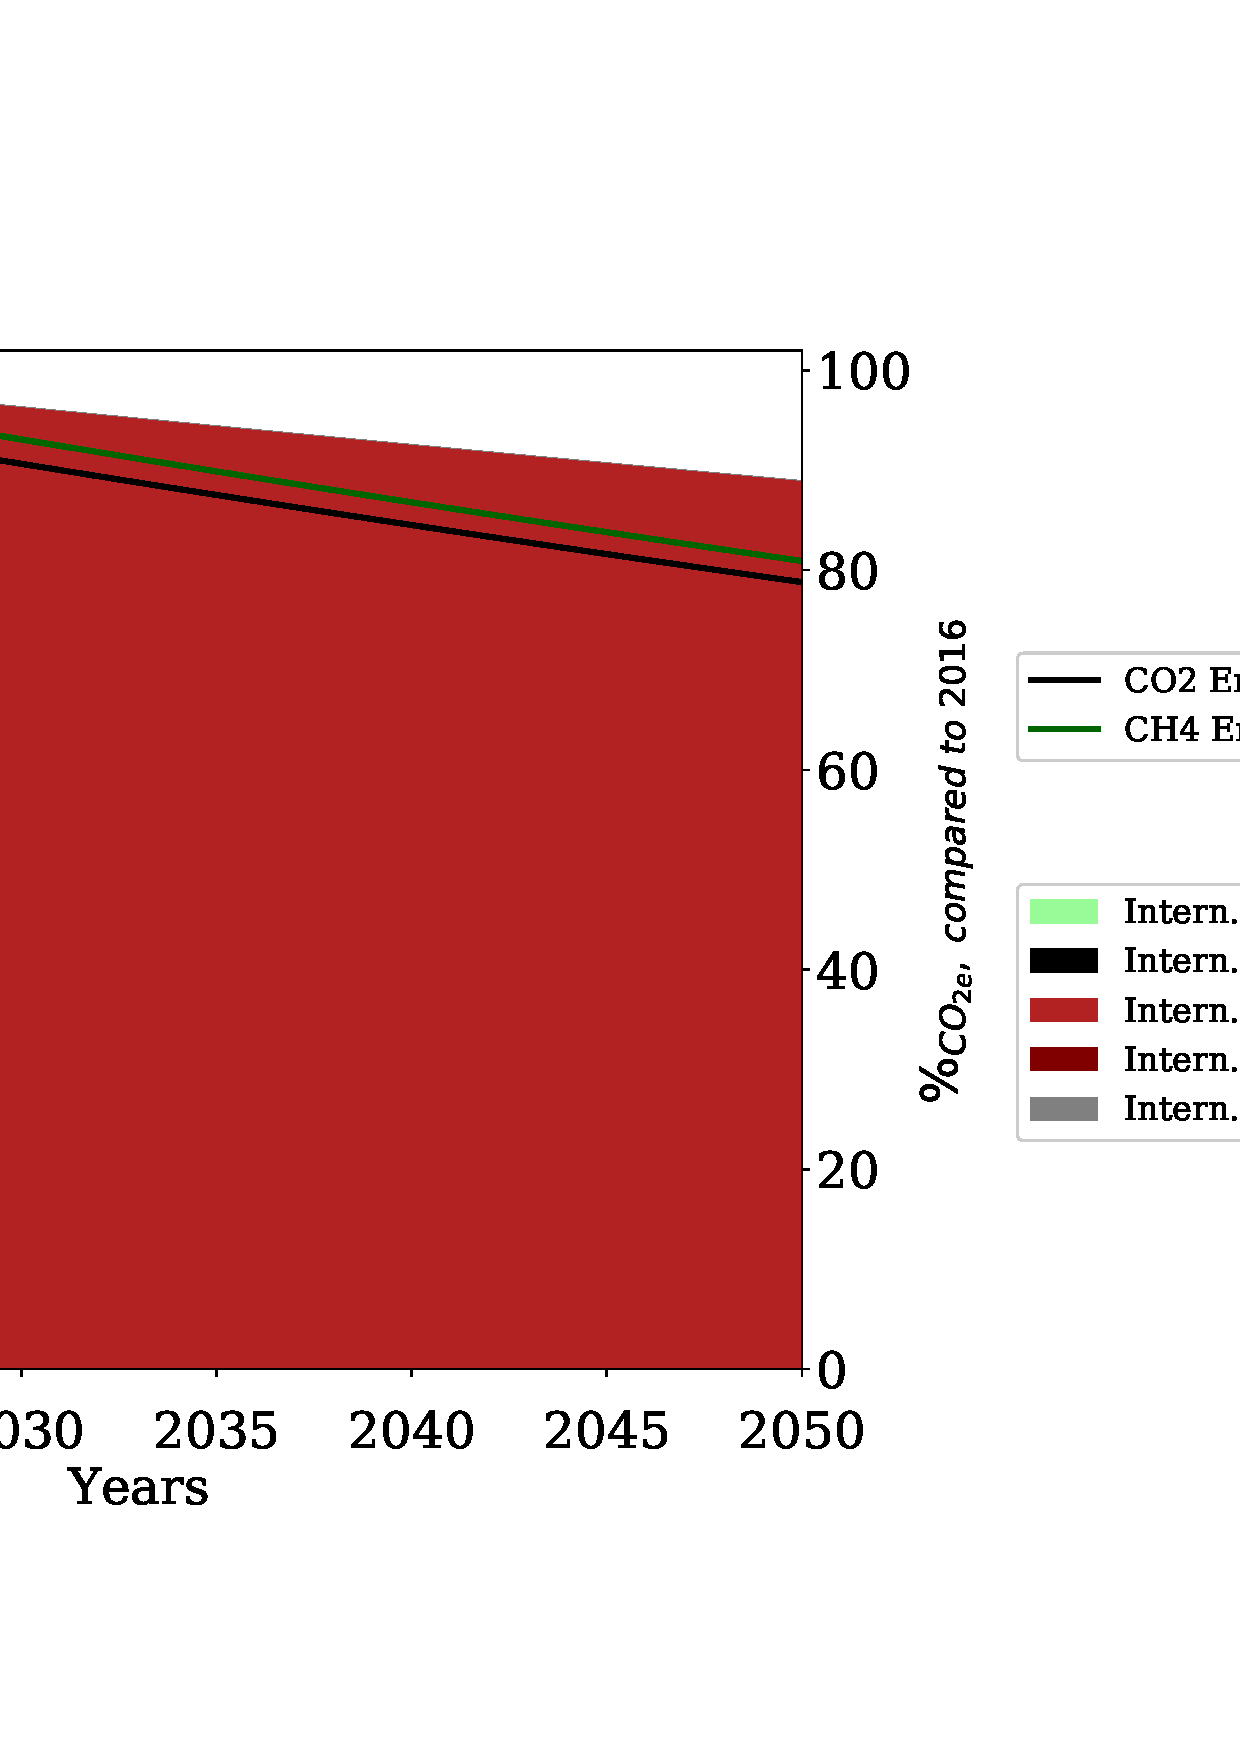
\includegraphics[width=\textwidth]{figures/BAU_fuels_emissions.pdf}
    \caption{Fuel consumption (y-axis left) and cumulative emissions (y-axis right) in the Business-as-usual scenario without carbon budget}
    \label{fig:BAU}
    % TODO: Figure einfügen und am besten auf einer zweiten y-Achse die kumulativen Emissionen reinbringen. Die fuels vll. einfach in % angeben, falls das mit den 16PJ nicht mehr herauszubekommen ist.
\end{figure}

\begin{figure}[htb]
    \centering
    \includegraphics[width=\textwidth]{figures/IMO_fuels_emissions.pdf}
    \caption{Fuel consumption (y-axis left) and cumulative emissions (y-axis right) in the IMO scenario, applying the climate emission target of the International Maritime Organsiation for 2050}
    \label{fig:IMO}
    % TODO: Figure einfügen und am besten auf einer zweiten y-Achse die kumulativen Emissionen reinbringen. Die fuels vll. einfach in % angeben, falls das mit den 16PJ nicht mehr herauszubekommen ist.
\end{figure}

\begin{figure}[htb]
    \centering
    \includegraphics[width=\textwidth]{figures/REF_fuels_emissions.pdf}
    \caption{Fuel consumption (y-axis left) and cumulative emissions (y-axis right) in the Reference scenario with a limited carbon budget}
    \label{fig:REF}
    % TODO: Figure einfügen und am besten auf einer zweiten y-Achse die kumulativen Emissionen reinbringen. Die fuels vll. einfach in % angeben, falls das mit den 16PJ nicht mehr herauszubekommen ist.
\end{figure}

% REF compared to REF methane leakage?


% Cost variation: Methanol and Ammonia are close
Due to the high level of uncertainty of cost development of infrastructure, fuel and propulsion technology of different marine fuel options, a wide range of cost variations is applied to test for its effect on fuel composition. The results are summarised in \autoref{fig:costVariation}. Depending on the cost rate change of a specific fuel (x-axis), its share in the total fuel consumption from 2016-2050 (y-axis) changes significantly. The black dashed line at a cost rate change of zero represents the reference scenario. Already at a change of 10\% cost change rate (including fuel, technology and infrastructure costs), methanol and ammonia gain relevance, reaching a dominant role at a 20\% cost change rate.

% LNG is no option, LBG just if methane leakage phase out
For LBG, the development of the methane leakage problem is of outstanding importance. Under the assumption that methane leakage can be coped with until 2050 (dashed line), LBG is close to hydrogen, methanol and ammonia as choice to be the dominate fuel in 2050. Contrary to that, LNG would not only require a methane leakage phase out, but also a very favourable cost development to play a major role.

% BATW has to be decreased significantly, but the conditions applied were rather unfavorable for BATW.


\begin{figure}[htb]
    \centering
    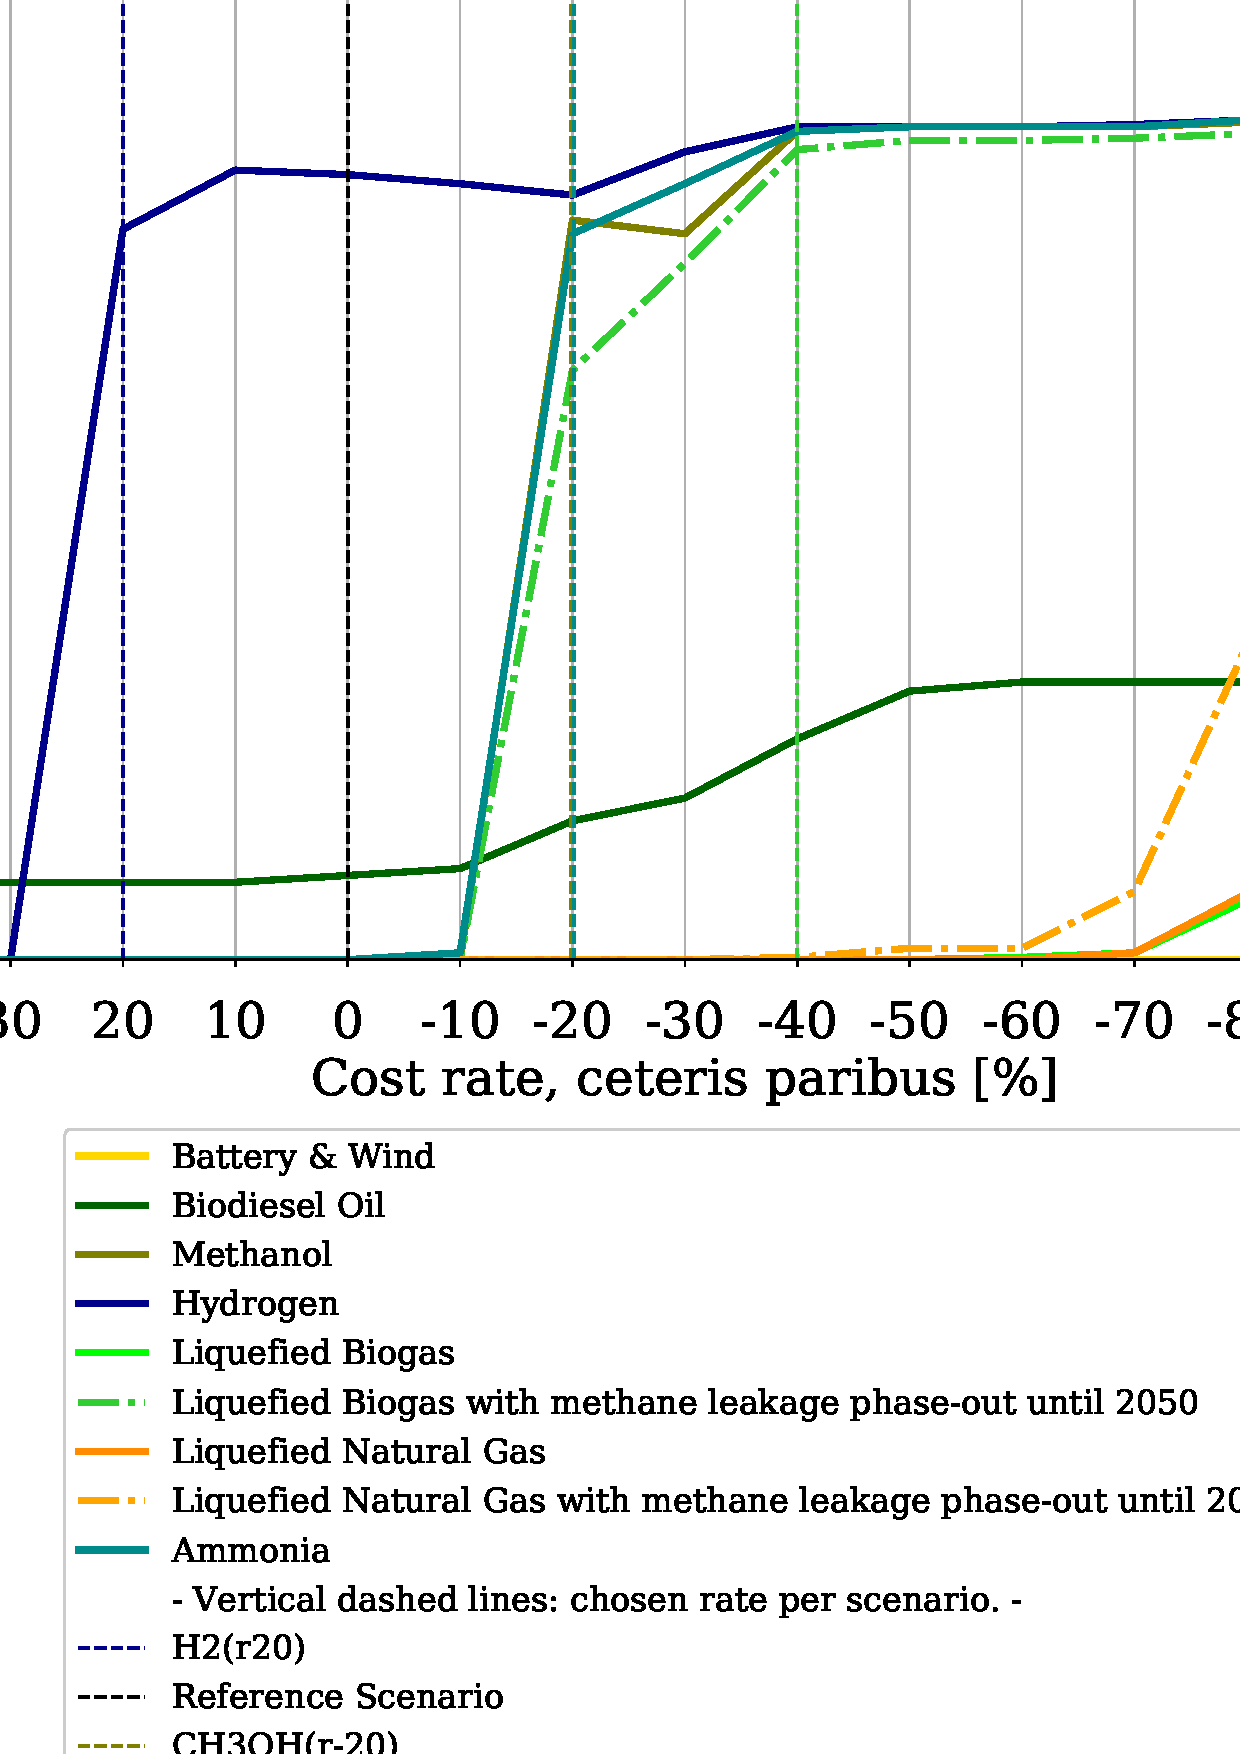
\includegraphics[width=\textwidth]{figures/costVariation.pdf}
    \caption{Total fuel shares from 2016-2050 (y-axis) in relation to different cost range changes (x-axis) compared to the reference case}
    \label{fig:costVariation}
    % TODO: Figure einfügen mit ausfuehrlicheren Fuel Namen
\end{figure}


% NOTES:
Figures:
\begin{itemize}
    \item Cost variation curve and its effect: When comes what in
    \item Fuel comparison of all scenarios: Fuel composition in 2050 (relative or absolut?)
    \item Maybe emission reduction over time for all scenarios (maybe including methane leakage)
\end{itemize}


Key findings:
\begin{itemize}
    \item It seems possible to become CO2e-neutral by 2050 with existing technologies
    \item Carbon price of 350 to 450 Euro/tCO2 necessary
    \item Transport costs increase on average by 6\% per cargo value
    \item H2, CH3OH and NH3 most compatible, no clear winner
    \item LBG needs significant reduction of methane leakage to be attractive option for climate and from socio-economic perspective.
    \item LNG s not an option due to costs and carbon emissions.
    \item Battery + wind could be if...
\end{itemize}

\section{Conclusion}
% 250 words
% only draft until now!
For the possibility to reach the ..., it is of great importance, that the shipping sector becomes CO2-neutral. It is possible for the Danish part of international shipping to become CO2-neutral until 2050 with existing technologies. H2, CH3OH and NH3 seem from today to be most compatible while there is no clear winner. Which one would be the best option from a soico-economic point of view will depend mainly on the cost development. For ammonia also safety. All would be applied in Fuel Cells due to its higher fuel efficiency. LNG is no option due to a short window of opportunity and its leakage problem. LBG only if a very optimistic pathway of methane leakage reduction is assumed. Battery and wind could be an option for the long range, but that is not fully displayed in the modelling configuration. Safety issues, infrastructure decisisons, questions of the transformation require a more detailed attempt.
However, gives and indication, that either strong targets/carbon budgets or a carbon price of 350-450 EURO/TCO2 would be required to induce the changes. This would double the costs for cargo, but due to its low share on cargo value, on average only 6\% of the cargo value.

\section*{References}

\bibliography{mybibfile}

\end{document}